\documentclass[11pt]{article}

\usepackage[T1]{fontenc}
\usepackage{lmodern}
\usepackage[margin=1in]{geometry}
\usepackage{microtype}
\usepackage{amsmath,amssymb,amsthm}
\usepackage{booktabs}
\usepackage{array}
\usepackage{enumitem}
\usepackage{tikz}
\usepackage{xcolor}
\usepackage{xurl}
\usepackage[hidelinks]{hyperref}

\newtheorem{theorem}{Theorem}
\newtheorem{lemma}[theorem]{Lemma}
\newtheorem{proposition}[theorem]{Proposition}
\theoremstyle{definition}
\newtheorem{definition}[theorem]{Definition}
\theoremstyle{remark}
\newtheorem{remark}[theorem]{Remark}

\newcommand{\Q}{Q}
\newcommand{\interior}{\operatorname{int}}
\newcommand{\abs}[1]{\left|#1\right|}
\newcommand{\norminf}[1]{\left\lVert #1\right\rVert_{\infty}}

\title{An Exact Computer-Assisted Lower Bound for\\Packing 17 Unit Squares in a Square}
\author{Mira\\\small \url{https://github.com/Mira-acc/17squares}}
\date{September 2026}

\hypersetup{
  pdftitle={An Exact Computer-Assisted Lower Bound for Packing 17 Unit Squares in a Square},
  pdfauthor={Mira},
  pdfsubject={Computer-assisted discrete geometry},
  pdfkeywords={square packing, unavoidable points, computer-assisted proof, exact arithmetic}
}

\begin{document}
\maketitle
\begin{abstract}
Let $s(17)$ be the least side length of a square containing seventeen pairwise
interior-disjoint unit squares, with arbitrary orientations. We give an exact
computer-assisted certificate proving $s(17)>4.613028635886$. A nonnegative
rational measure on 1,620 points has total mass $16.99798498<17$, yet assigns
mass at least one to the interior of every contained unit square. An exact
sweep verifies all translations of smaller closed cores at 2,881 directions;
a strict containment inequality covers the intervening orientations. Rational
scaling gives a slightly larger radical lower bound with a weak inequality.
The two accumulation engines share one geometric kernel. The earlier
sixteen-point proof of $s(17)>4.468292$ is retained in an appendix.
\end{abstract}

\section{Result and provenance}
Write $\Q_L=[0,L]^2$. Squares in a packing may touch, but their interiors must
be disjoint. The minimum defining $s(17)$ is attained: centres and orientations
range over a compact parameter space, and containment and nonoverlap are closed
conditions.
\begin{theorem}\label{thm:main}
Let
\[
 L=\frac{4613}{1000},\quad B=\frac{19997}{20000},\quad
 h=\frac{207107}{1440000000}.
\]
Then
\[
 s(17)\ge S_*:=\frac{L\sqrt{1+h^2}}{B(1+h)}
 =\sqrt{\frac{17650291964463886688094912400}{829429719507765981945905041}}
 >4.613028635886.
\]
\end{theorem}
The base certificate excludes a packing at side $4.613$. The endpoint
$S_*=4.613028635886110\ldots$ follows by dilation; exclusion at that endpoint
is not asserted. The cited upper-bound construction is
Bidwell's packing, of side about $4.67553009360455$\cite{Friedman2009,Ellsworth2026}.
Thus the resulting interval is
\[
 4.613028635886<s(17)\le4.67553009360455\ldots.
\]
This is a claim about the supplied certificate and cited comparison data,
not an exhaustive assertion of priority over other work.

The starting 1,184-atom certificate at side $4.59$ is due to Joshua Levy's
\emph{squares} project\cite{Levy17}. The weighted covering principle and
covering linear-program strategy predate this calculation, and the sharp
dilation lemma used below is credited to Levy's T-022 note\cite{LevyDilation}.
The preceding weighted certificate proved $s(17)>4.607028598640$.
The present continuation raises its base side from $4.607$ to $4.613$ by
changing the spatial support and weights. The core side, direction net and
exact geometric kernel are unchanged. The earlier certificate and its
Levy/Mira support provenance remain in \path{certificates/lower_bound_4p607/}.
The new certificate has 206 positive symmetry orbits, expanding to 1,620 atoms.

\section{Weighted interior coverage}
Let $\mu=\sum_j w_j\delta_{p_j}$, where $p_j\in\Q_L$ and $w_j\ge0$ are rational.
If $\mu(\Q_L)<17$ and $\mu(\interior U)\ge1$ for every contained unit square
$U$, then seventeen interior-disjoint such squares would have total interior
mass at least 17 and at most $\mu(\Q_L)$, a contradiction. Sixteen unavoidable
points, each of weight one, are the historical special case in the appendix.

The new certificate is invariant under the eight symmetries $D_4$ of $\Q_L$.
This restricts the measure, not a hypothetical packing. Set
\[
 T=\frac{207107}{500000},\quad m=2880,\quad
 t_k=\frac{kT}{m},\quad\theta_k=2\arctan t_k\quad(0\le k\le m).
\]
The checker verifies nonnegative weights, atom containment, $D_4$ invariance,
total mass below 17, and
\begin{equation}\label{eq:angular}
 T^2+2T\ge1,\qquad B^2(1+h)^2<1+h^2,\qquad h=T/m<1.
\end{equation}
It then checks that every closed side-$B$ square contained in $\Q_L$ at each
$\theta_k$ has mass at least one.

Container symmetries and square symmetries reduce any individual orientation
to $[0,\pi/4]$. The first inequality in \eqref{eq:angular} ensures that the
net reaches this interval's upper endpoint. For the nearest net angle, the
angular distance $\delta$ satisfies
\[
 \tan\delta\le\frac{t_{k+1}-t_k}{1+t_kt_{k+1}}\le h.
\]
For $0\le z\le h<1$ the identity
\[
 (1+h)^2(1+z^2)-(1+z)^2(1+h^2)=2(h-z)(1-hz)\ge0
\]
gives $\cos\delta+\sin\delta\le(1+h)/\sqrt{1+h^2}$. Therefore a concentric
closed side-$B$ core at the chosen net angle has projections strictly smaller
than one on both axes of the unit square. It lies strictly inside that square,
and hence inside the container. Its mass is at least one by the finite check.
Atoms on a core boundary are still strictly inside the parent unit square,
so touching unit squares cannot double-count them.

\section{Checking every translation exactly}
Centre the container at the origin. At a net angle let $c=\cos\theta>0$ and
$s=\sin\theta\ge0$. The admissible core centres form $[-H,H]^2$, where
$H=(L-B(c+s))/2$. The checker requires $H>0$ at every direction.
In rotated coordinates $u=cx+sy$, $v=-sx+cy$, the centre domain is
\[
 D=\{(u,v):|cu-sv|\le H,\ |su+cv|\le H\}.
\]
An atom contributes its weight on a closed axis-parallel rectangle of side
$B$ centred at its rotated coordinates. Rectangle edges and the extreme
$u$ coordinates of $D$ partition the plane into open cells of constant mass.

For each open $u$ slab $(a,b)$ intersecting the interior of $D$, the projection
of that intersection on the $v$ axis is an open interval $(v_{\min},v_{\max})$.
When $s>0$, the lower and upper boundaries of $D$ are
\[
 \ell(u)=\max\left\{\frac{cu-H}{s},\frac{-H-su}{c}\right\},\quad
 r(u)=\min\left\{\frac{cu+H}{s},\frac{H-su}{c}\right\}.
\]
Their minimum and maximum occur at $u=H(c-s)$ and $u=-H(c-s)$, respectively,
clamped to $[a,b]$. These evaluations give $v_{\min}$ and $v_{\max}$;
for $s=0$ they are $-H,H$. A $v$ cell is reachable exactly when its open
interval overlaps $(v_{\min},v_{\max})$. A range-minimum sweep checks its mass.

Boundary placements also have mass at least one. Each is a limit of interior
placements avoiding all event lines. There are finitely many cells, so a
subsequence lies in one fixed cell. Each atom captured there remains captured
at the limit because core membership is closed. Nonnegative weights imply
that mass cannot decrease at this boundary. This covers wall contacts,
coincident events and vertices, completing the translation argument.

\subsection{Integer representation and trust boundary}
For a reduced half-tangent $p/q$ put
\[
 C=q^2-p^2,\quad S=2pq,\quad R=q^2+p^2,
 \qquad c=C/R,\quad s=S/R.
\]
Choose an integer scale $G$ making centred atom coordinates $X_j,Y_j$,
$\ell_0=GL/2$ and $b_0=GB/2$ integral. In units $1/(R^2G)$ the projected
atom coordinates and rectangle half-width are
\[
 U_j=R(CX_j+SY_j),\quad V_j=R(-SX_j+CY_j),\quad J=b_0R^2.
\]
With $H_0=\ell_0R-b_0(C+S)$, the domain inequalities are
$|CU-SV|\le R^2H_0$ and $|SU+CV|\le R^2H_0$.
All geometry and rational comparisons use unbounded Boost integers.
Weights use a common denominator; the checker caps the summed integer
numerators at $10^{12}$ to protect signed 64-bit accumulation.

A segment tree and a direct difference-array/prefix-sum engine evaluate the
same geometric cells. Their complete logs must agree. This audits two
implementations of accumulation, not two independently authored geometric
proofs. The JSON input compiler preserves rationals exactly. The numerical
optimizer and its sampled constraints are outside the trusted proof core.

\section{Dilation and reproducibility}
Put $C_0=\sqrt{1+h^2}/(B(1+h))>1$. For every rational $0<r<C_0$, scale the
container, cores and atom coordinates by $r$, leaving weights unchanged.
Inverse scaling preserves core coverage and the scaled cores still satisfy
the strict angular inequality. The weighted contradiction excludes a packing
at side $rL$. Taking rational $r$ increasing to $C_0$ proves $s(17)\ge S_*$.
The exact rational comparison $(4.613028635886)^2<S_*^2$ proves the strict
decimal statement in Theorem~\ref{thm:main}. At $C_0$ the containment inequality
becomes equality, which is why the endpoint statement remains weak.

\begin{center}
\begin{tabular}{lr}
\toprule
Certificate quantity & Exact value\\
\midrule
Atoms & 1,620\\
Directions & 2,881\\
Total mass & $849899249/50000000=16.99798498$\\
Minimum closed-core mass & $1000002103/1000000000=1.000002103$\\
Centre slabs & 9,116,871\\
\bottomrule
\end{tabular}
\end{center}
The authoritative atoms are in
\path{certificates/lower_bound_4p613/best-certificate.json}, with SHA-256
\begin{center}\small\ttfamily
749f13335980a66a27a2304f212b5d8796390c81b962149647a4d9ff43a228ec.
\end{center}
From the repository root, run
\begin{quote}\ttfamily\small
python3 certificates/lower\_bound\_4p613/verify.py --source
\end{quote}
This rebuilds both engines, runs thirteen positive/refusal controls per engine,
replays the pinned Levy source and new certificate, compares logs, and checks
the result ledger and endpoint. It also runs eight controls for the exact
dictionary diagnostic and reconstructs the orbit-deletion experiment in both
engines. Python 3.10 or newer with its standard library, C++17 and Boost
headers suffice. The command \texttt{bash ./verify\_all.sh} additionally
replays the preceding weighted certificate and regenerates and checks the
historical triangle-witness certificate.
The weighted package has its own SHA-256 manifest; the historical package
retains its original raw and compressed certificate hashes.

\section{Spatial search and exact diagnostics}
The search alternates between adding under-covered core placements as
constraints and using linear-program dual multipliers to propose new point
orbits. Final normalization and upward rational rounding produce the measure
checked above. These numerical operations suggest data; the full exact replay
establishes coverage without assuming numerical feasibility or optimality.
An unsuccessful search at side $4.615$ supplied some useful support geometry
for the final $4.613$ run, but supplies no theorem at $4.615$.

Two exact diagnostics explain the role of the new sites. For a prescribed
356-orbit dictionary at side $4.61$, the package gives 106 contained rational
cores $C_i$ and nonnegative rational multipliers $z_i$. If
$A_{ij}=|O_j\cap C_i|$, the diagnostic checks
\[
 \sum_i z_iA_{ij}\le|O_j|\quad\text{for every prescribed orbit }O_j,
 \qquad \sum_i z_i=17.009583872717.
\]
Any nonnegative per-atom orbit weights $w_j$ covering these cores must satisfy
\[
 \sum_j|O_j|w_j\ge\sum_i z_i\sum_j A_{ij}w_j
 \ge\sum_i z_i>17.
\]
Thus reweighting this dictionary cannot pass the specified core test at $4.61$.
The conclusion does not constrain other supports or verification methods.
The diagnostic recomputes core containment, incidences and dual inequalities
using integers and exact fractions; it does not trust a stored incidence matrix.

Separately, the orbit ledger reconstructs the final accepted measure exactly.
Deleting its 19 final-stage priced orbits removes 152 atoms of total mass
$0.315664656$. The remaining mass is $16.682320324$, and exact replay rejects
at direction zero with core minimum $0.939043209$. Uniform rescaling to repair
that minimum would exceed mass 17. This concerns deletion from this fixed
certificate; reoptimization without those orbits is not ruled out.

\paragraph{Attribution and status.}
Levy's original and the derived certificate data are credited under CC BY 4.0;
source hashes and changes are recorded in the package's \path{ATTRIBUTION.md}.
This is a computer-assisted working preprint, with external peer review pending.
The earlier computation and exposition were developed with assistance from
OpenAI's GPT-5.6 Pro under human direction; the September patch and this
integration also used AI assistance. The claim rests on the explicit data,
mathematical reduction and executable checker. No optimality of the measure
or the cited upper bound is asserted.

\clearpage
\appendix
\suppressfloats[t]
\section{Historical triangle-witness theorem}
The August certificate proves the following earlier result. Throughout this
appendix, $L=4468292/1000000=4.468292$.
\begin{theorem}\label{thm:historical}
No packing of seventeen unit squares exists in $\Q_L$. Consequently,
$s(17)>4.468292$.
\end{theorem}
The preceding exact point-witness bound was $s(17)>4.456575$, due to
Fort\cite{Fort2026}. This certificate improves it by $0.011717$ and adds
orientation-independent triangle witnesses to the subdivision language.
The historical data and three checkers remain in
\path{certificates/lower_bound_4p468292/}.

\section{Strictly unavoidable points}

\begin{definition}
A finite set $P\subseteq \Q_L$ is \emph{strictly unavoidable for unit squares}
if every unit square $U\subseteq \Q_L$ satisfies
\[
  P\cap\interior(U)\ne\varnothing.
\]
\end{definition}

\begin{lemma}[Pigeonhole lemma]\label{lem:pigeonhole}
If $\Q_L$ contains a strictly unavoidable set of $n-1$ points, then no packing
of $n$ pairwise interior-disjoint unit squares exists in $\Q_L$.
\end{lemma}

\begin{proof}
Suppose $U_1,\dots,U_n$ were such a packing.  For each $i$, choose
$p_i\in P\cap\interior(U_i)$.  If $p_i=p_j$ for $i\ne j$, then that point lies
in both square interiors, contradicting interior-disjointness.  Thus the map
$i\mapsto p_i$ is an injection from an $n$-element set into an $(n-1)$-element
set, which is impossible.
\end{proof}

The use of interiors is important.  Boundary witnesses could be shared by
several touching squares and would not imply the injection in
Lemma~\ref{lem:pigeonhole}.

For Theorem~\ref{thm:historical}, the set $P$ consists of the sixteen rational points
in Table~\ref{tab:points}.  Every displayed decimal is exact, with denominator
$10^7$.

\begin{table}[t]
\centering
\caption{The sixteen rational witness points.}
\label{tab:points}
\small
\setlength{\tabcolsep}{8pt}
\begin{tabular}{rcc@{\qquad}rcc}
\toprule
$i$ & $x_i$ & $y_i$ & $i$ & $x_i$ & $y_i$\\
\midrule
 1 & 0.9633740 & 0.9849850 &  9 & 0.9172158 & 2.6508741\\
 2 & 1.6317845 & 0.9829523 & 10 & 1.4694893 & 2.6410332\\
 3 & 2.5287879 & 0.9446006 & 11 & 2.4689011 & 2.6753176\\
 4 & 3.4682923 & 0.9443212 & 12 & 3.4682923 & 2.7101964\\
 5 & 0.9999997 & 1.7580956 & 13 & 0.9999997 & 3.5239708\\
 6 & 1.9993909 & 1.7929744 & 14 & 1.9395041 & 3.5236914\\
 7 & 2.9988027 & 1.8272588 & 15 & 2.8365087 & 3.4853407\\
 8 & 3.5451063 & 1.8219620 & 16 & 3.4687946 & 3.4687946\\
\bottomrule
\end{tabular}
\end{table}

\begin{figure}[t]
\centering
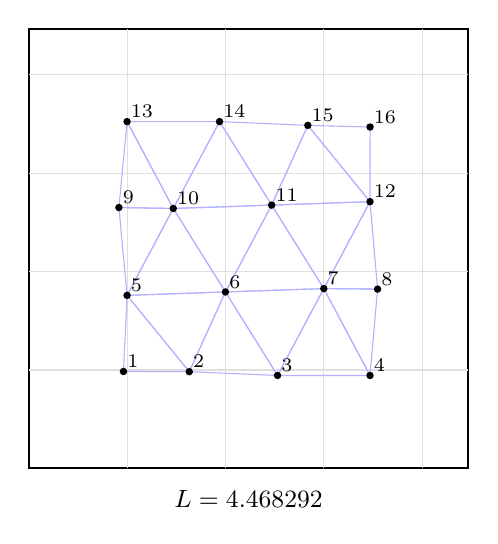
\begin{tikzpicture}[x=1.25cm,y=1.25cm]
  \draw[line width=0.7pt] (0,0) rectangle (4.468292,4.468292);
  \foreach \g in {1,2,3,4} {
    \draw[gray!25,thin] (\g,0) -- (\g,4.468292);
    \draw[gray!25,thin] (0,\g) -- (4.468292,\g);
  }
  \coordinate (p1) at (0.9633740,0.9849850);
  \coordinate (p2) at (1.6317845,0.9829523);
  \coordinate (p3) at (2.5287879,0.9446006);
  \coordinate (p4) at (3.4682923,0.9443212);
  \coordinate (p5) at (0.9999997,1.7580956);
  \coordinate (p6) at (1.9993909,1.7929744);
  \coordinate (p7) at (2.9988027,1.8272588);
  \coordinate (p8) at (3.5451063,1.8219620);
  \coordinate (p9) at (0.9172158,2.6508741);
  \coordinate (p10) at (1.4694893,2.6410332);
  \coordinate (p11) at (2.4689011,2.6753176);
  \coordinate (p12) at (3.4682923,2.7101964);
  \coordinate (p13) at (0.9999997,3.5239708);
  \coordinate (p14) at (1.9395041,3.5236914);
  \coordinate (p15) at (2.8365087,3.4853407);
  \coordinate (p16) at (3.4687946,3.4687946);
  \foreach \a/\b/\c in {
    1/2/5,2/3/6,2/5/6,3/4/7,3/6/7,4/7/8,
    5/6/10,5/9/10,6/7/11,6/10/11,7/8/12,7/11/12,
    9/10/13,10/11/14,10/13/14,11/12/15,11/14/15,12/15/16}
    \draw[blue!30,thin] (p\a) -- (p\b) -- (p\c) -- cycle;
  \foreach \x/\y/\n in {
    0.9633740/0.9849850/1,1.6317845/0.9829523/2,
    2.5287879/0.9446006/3,3.4682923/0.9443212/4,
    0.9999997/1.7580956/5,1.9993909/1.7929744/6,
    2.9988027/1.8272588/7,3.5451063/1.8219620/8,
    0.9172158/2.6508741/9,1.4694893/2.6410332/10,
    2.4689011/2.6753176/11,3.4682923/2.7101964/12,
    0.9999997/3.5239708/13,1.9395041/3.5236914/14,
    2.8365087/3.4853407/15,3.4687946/3.4687946/16}
  {
    \fill (\x,\y) circle[radius=1.35pt];
    \node[font=\scriptsize,anchor=south west,inner sep=1.2pt] at (\x,\y) {\n};
  }
  \node[font=\small,anchor=north] at (2.234146,-0.12) {$L=4.468292$};
\end{tikzpicture}
\caption{The witness set and the eighteen certified triangles.  The proof uses
the exact rational coordinates in Table~\ref{tab:points}; blue edges indicate
the orientation-independent triangle witnesses.}
\label{fig:points}
\end{figure}

\section{Parameterizing a unit square}

A unit square is unchanged by a rotation through $\pi/2$.  We may therefore
represent every orientation by an angle
\[
  -\frac{\pi}{4}\le \theta\le\frac{\pi}{4},
  \qquad t=\tan\theta\in[-1,1].
\]
Let $(x,y)$ be the center of the square, and let $p=(p_x,p_y)$ be a fixed
point.  Put
\[
  \Delta x=p_x-x,\qquad \Delta y=p_y-y,
  \qquad r=\sqrt{1+t^2}.
\]
In coordinates aligned with the square, the displacement from the center to
$p$ is
\[
  \left(\frac{\Delta x+t\Delta y}{r},
        \frac{-t\Delta x+\Delta y}{r}\right).
\]
Consequently, $p$ lies strictly inside the square exactly when
\begin{align}
  4(\Delta x+t\Delta y)^2 &< 1+t^2,\label{eq:inside-a}\\
  4(-t\Delta x+\Delta y)^2 &< 1+t^2.\label{eq:inside-b}
\end{align}

The axis-parallel half-extent of a unit square with parameter $t$ is
\[
  h(t)=\frac{1+\abs{t}}{2\sqrt{1+t^2}}.
\]
Thus containment in $\Q_L$ requires
\[
  h(t)\le x,y\le L-h(t).
\]
The function $u\mapsto(1+u)/(2\sqrt{1+u^2})$ is nondecreasing on $[0,1]$.
This monotonicity supplies a simple exact test for pose boxes that cannot
contain any feasible square.

\section{The subdivision certificate}\label{sec:certificate}

The pose space is parameterized by $(x,y,t)$.  The checker begins with the
rational box
\[
  \mathcal B_0=
  \left[\frac12,L-\frac12\right]^2\times[-1,1],
\]
which contains every feasible pose.  It recursively bisects boxes in one of
the three coordinates.  Each node is encoded by one byte:

\begin{center}
\begin{tabular}{cl}
\toprule
Byte & Meaning\\
\midrule
$0$ & the current box contains no feasible square pose;\\
$1,\dots,16$ & the indicated point lies strictly inside every pose in the box;\\
$17,18,19$ & bisect the box in $x$, $y$, or $t$, respectively.\\
$20,\dots,37$ & the indicated triangle pierces every pose in the box.\\
\bottomrule
\end{tabular}
\end{center}

The verifier distrusts every leaf claim and recomputes it from the box
endpoints.

\subsection{Infeasible leaves}

For a box
\[
  \mathcal B=[x_0,x_1]\times[y_0,y_1]\times[t_0,t_1],
\]
let
\[
  u=\min\{\abs t:t\in[t_0,t_1]\}.
\]
Since $h(t)\ge h(u)$ throughout the box, the box is infeasible if any one of
\[
  x_1<h(u),\quad L-x_0<h(u),\quad
  y_1<h(u),\quad L-y_0<h(u)
\]
holds.  The checker clears denominators and squares nonnegative quantities, so
this test is performed using integers only.

\subsection{Point-witness leaves}

Fix a witness point $p$.  Exact interval arithmetic over $\mathcal B$ gives
intervals containing
\[
  A=\Delta x+t\Delta y,
  \qquad B=-t\Delta x+\Delta y.
\]
Write $M_A$ and $M_B$ for the maximum absolute endpoint of these intervals.
Because $1+t^2\ge1+u^2$ throughout the box, the two strict inequalities
\[
  4M_A^2<1+u^2,
  \qquad 4M_B^2<1+u^2
\]
prove simultaneously that $p$ is strictly inside every square represented by
that box.  Again, the implementation stores rational endpoints on fixed grids
and clears every denominator before comparison.

The interval enclosure for the bilinear term $t\Delta y$ is obtained by taking
the minimum and maximum of its four corner products; the same is done for
$(-t)\Delta x$.  No floating-point approximation enters a leaf decision.

\subsection{Triangle-witness leaves}

Some center boxes can be closed without subdividing the orientation interval.
The certificate fixes eighteen triangles whose vertices belong to the witness
set and applies the following lemma.

\begin{lemma}[Strict triangle piercing]\label{lem:triangle}
Let $A,B,C$ be three points whose pairwise distances are strictly less than
one.  Every unit square whose center lies strictly inside triangle $ABC$
contains at least one of $A,B,C$ strictly in its interior.
\end{lemma}

\begin{proof}
Translate the square center to the origin and rotate the plane so the square is
$[-1/2,1/2]^2$.  Its diagonals divide the plane into right, top, left, and
bottom closed cones.  Because the origin lies strictly inside triangle $ABC$,
the three vertices cannot all lie in a closed half-plane bounded by either
diagonal.  Among the four cones this forces two vertices into opposite cones.
If neither vertex were in
the square interior, vertices in the right and left cones would have
$x$-coordinates differing by at least one; vertices in the top and bottom
cones would have $y$-coordinates differing by at least one.  In either case
their Euclidean distance would be at least one, contradicting the strict
side-length hypothesis.
\end{proof}

For a triangle leaf, the checker first verifies the three strict inequalities
\[
  \lVert A-B\rVert_2^2<1,\qquad
  \lVert B-C\rVert_2^2<1,\qquad
  \lVert C-A\rVert_2^2<1.
\]
It orients the triangle counterclockwise and checks that all four corners of
the center rectangle lie strictly to the left of each directed edge.  Each
edge test is affine in the center coordinates, so positivity at the four
corners proves positivity throughout the rectangle.  Lemma~\ref{lem:triangle}
then covers every orientation in the box.  The checker clears denominators and
performs these tests with integers only.

\subsection{Completeness of the tree}

The checker traverses the tree from $\mathcal B_0$, applying every split exactly.
It rejects an early end of file, an unknown opcode, a false leaf claim, or any
trailing byte.  Finally it checks the full-binary-tree identity
\[
  \#\text{leaves}=\#\text{split nodes}+1.
\]
It follows inductively that the accepted leaves form a cover of the complete
root box.  Every feasible pose is therefore covered by either a point-witness
leaf or a triangle-witness leaf.  In both cases at least one of the sixteen
points lies strictly inside the square, so the point set is strictly
unavoidable.

Lemma~\ref{lem:pigeonhole} now rules out a packing in $\Q_L$, and therefore in
every smaller container as well.  Thus $s(17)\ge L$.  The minimum defining
$s(17)$ is attained by compactness, so equality would give a packing in
$\Q_L$.  Hence $s(17)>L$, proving Theorem~\ref{thm:historical}.

\section{Exact arithmetic and reproducibility}

The certificate uses the scales
\[
  S_t=2^{40},\qquad S_x=10^6\,2^{40},\qquad D_p=10^7.
\]
The center and slope endpoints are stored as integers on these fixed rational
grids, while the witness points have denominator $D_p$.  The accepted tree has
\begin{center}
\begin{tabular}{lr}
\toprule
Total nodes & $122{,}626{,}747$\\
Split nodes & $61{,}313{,}373$\\
Point-witness leaves & $33{,}762{,}069$\\
Triangle-witness leaves & $483{,}875$\\
Infeasible leaves & $27{,}067{,}430$\\
Maximum depth & $74$\\
\bottomrule
\end{tabular}
\end{center}
The certificate consists of one byte per node.  Its raw SHA-256 digest is
\begin{center}
\small\ttfamily
2838f315302d67da131745925e9ec7dd2a602bb299d1335ce25e4e13a7b7b6d2.
\end{center}
The raw tree is $122{,}626{,}747$ bytes, above GitHub's ordinary per-file
limit.  The repository stores a deterministic $374{,}096$-byte XZ archive with
SHA-256
\begin{center}
\small\ttfamily
a349b81e630ccf7292ae0afe6ed954591f7e88fe6289847f67883204a7ed60ac.
\end{center}

The repository provides three checkers:
\begin{enumerate}[leftmargin=2em]
  \item a fast C++ checker using bounded wide integers and the same arithmetic
    header as the generator;
  \item a separately implemented C++ checker using arbitrary-precision integers;
  \item a separately implemented Python checker using arbitrary-precision integers.
\end{enumerate}
The generator and its search heuristics are not part of the trusted proof core:
each checker reads the certificate as untrusted input and recomputes every leaf
claim.  The two arbitrary-precision checkers do not reuse the generator's
arithmetic routines, and so do not rely on a fixed-width overflow analysis.
From the repository root, the command
\begin{center}
\ttfamily bash ./verify\_all.sh
\end{center}
replays the weighted certificate and regenerates the historical certificate,
checks its hash, compares it byte-for-byte with the archive, and executes the
three historical verifiers.  The proof
package is available at
\url{https://github.com/Mira-acc/17squares}.

\begin{thebibliography}{9}

\bibitem{Friedman2009}
E. Friedman,
\newblock Packing unit squares in squares: A survey and new results,
\newblock \emph{Electron. J. Combin.}, Dynamic Survey DS7 (2009),
  first published 1998.
\newblock \url{https://doi.org/10.37236/28}.

\bibitem{Stromquist2003}
W. Stromquist,
\newblock Packing 10 or 11 unit squares in a square,
\newblock \emph{Electron. J. Combin.} 10(1) (2003), R8.
\newblock \url{https://doi.org/10.37236/1701}.

\bibitem{Ellsworth2026}
D. Ellsworth,
\newblock Squares in squares,
\newblock high-precision online packing catalogue, accessed 5 August 2026.
\newblock \url{https://kingbird.myphotos.cc/packing/squares_in_squares.html}.

\bibitem{Levy17}
J. Levy, the squares project,
\newblock Rational weighted certificate for seventeen squares.
\newblock Source data retained with Git blob
\texttt{f454e44dee1f2318af45e02efdfff5fcd7dbfbe1}.
\newblock \url{https://github.com/jlevy/squares/tree/main/packing/cases/n17_fractional_certificate}.

\bibitem{LevyDilation}
J. Levy, the squares project,
\newblock T-022: Dilation-limit proof for the eleven-square certificate.
\newblock \url{https://github.com/jlevy/squares/blob/main/packing/cases/n11_fractional_certificate/t-022-dilation-limit-proof.md}.
\bibitem{Fort2026}
S. Fort,
\newblock Packing 17 unit squares: exact lower bound $s(17)>4.456575$,
\newblock computer-assisted certificate repository (2026).
\newblock \url{https://github.com/stanislavfort/17squares}.

\end{thebibliography}

\end{document}
